\documentclass{article}
\usepackage{graphicx}
\usepackage{animate}
\usepackage{hyperref}
\usepackage{amsmath}
\usepackage[utf8]{inputenc}
\usepackage[style=alphabetic]{biblatex}
\addbibresource{references.bib}

\title{Draft: GSoC Julia PSO Application}
\author{Quazi Irfan \\ Mentors: Anthony Blaom, Sebastian Vollmer}
\date{April 2021}

\begin{document}

\tableofcontents
\maketitle

\section{Introduction}

Particle swarm optimization of Machine Learning models. Source:
\href{https://julialang.org/jsoc/gsoc/MLJ/#Particle-swarm-optimization-of-machine-learning-models}{Link to GSoC Idea}

\section{Particle Swarm Optimization in own words}

Particle Swarm Optimization is a nature inspired numerical optimization method to minimize a function by generating and manipulating a swarm of particle(that represents possible solutions) and improve those solutions iteratively by simulating the behaviour of a bird flocking or a fish schooling.

This algorithm starts with a set of candidate solution that are distributed over the space that is assumed to contain the minimum of the objective function. These candidate solutions are known as particles.

At each step of the algorithm, the particle tries to find a more optimal position for themselves. The position update rules can be expressed as the following expression, where $x(t)$ and $x(t+1)$ are vectors that represents all particle position at time $t$ and $t+1$ and $v(t+1)$ representing the velocity of the particle at time $t+1$.

\begin{equation}
x(t+1) = x(t) + v(t+1)
\end{equation}

As particles move, it records its own best position. Each particles also communicate with other particles in the swarm to find best position. At each iteration particle finds its next position using a combination of its personal best from the past and current swarm's best position. This continues until a stop condition is met.

The velocity update rule for each particle has a stochastic and deterministic part. The deterministic parts are the following,
\begin{enumerate}
\item Inertia component: The velocity of the particle($v(t)$) from last iteration multiplied by the inertia of the particle($w$). This serves as a memory of previous movement.
\item Personal component: The distance between the particle's past best position and current position($x_b - x(t)$). This terms makes the particle want to move back to his past best position. 
\item Social component: The distance between the swarm's best position and particle's current position($g_b - x(t)$).  This terms makes the particle want to move towards the swarm's best position.
\end{enumerate}

The personal and social component are multiplied by random values $r_1$ and $r_2$ that follows Uniform[0,1], and these terms introduces stochastic element to each particle movement. They are also multiplied by constant acceleration term $s_1$ and $s_2$. The inertia of the particle is also a constant term. 

The velocity update equation is the following,

\begin{equation}
v(t+1) = v(t)w + s_1 r_1(t)[x_b - x(t)] +  s_2 r_2(t)[g_b - x(t)]
\end{equation}

In each step of the algorithm, velocity is updated for each particle which is followed by position update. This process continues until a stopping condition is met. In my PSO implementation, I am ruining the algorithm for 25 iterations. Assuming unit time, my algorithm runs until $t=25$.

\subsection{Vanilla PSO implementation}

My vanilla PSO implementation can be found here, \cite{irfan_2021}. This implementation can minimizes a function of single variable. I'll demonstrate my PSO implementation by trying to optimize a single variable function, $f(x) = x^2$. Analytically we know that that the function minimizes at 0.

We will generate a swarm of 10 particles from -9 to 9 with interval 2. The graph of $f(x)$ is in blue and the swarm are represented as scatter point in unique colors(Iteration 0). The plot is an animation that will show the updated position of each particle on each iteration, from iteration 1 to 25. In the animated plot, we see a lot of oscillation in the first few iterations and the oscillation slowly dies down after each iteration. The particles are starting to converge after 15 iterations.  

This same observation is also evident in the cost history plot. On the x axis of the cost history graph we have the number of iteration and on y axis we have the average change in position in two successive iterations. Note that there is a spike in the cost history at the beginning since the initial velocity of the particles are zero and they get too excited by the global minimum resulting in overshooting it - this phenomenon is noticeable in iteration 3.

The values of particle position are also present in Table 1. As we can see that the particles are uniformly distribute at Iteration 0, and starts to converge in first few iterations, and by the 10th iteration they are already very close to our analytical solution. By 25th iteration all particles are very close to 0 - which is what we expect.

\animategraphics[loop,autoplay, width=\linewidth]{1}{./plots/plot}{0}{25}
\begin{center}
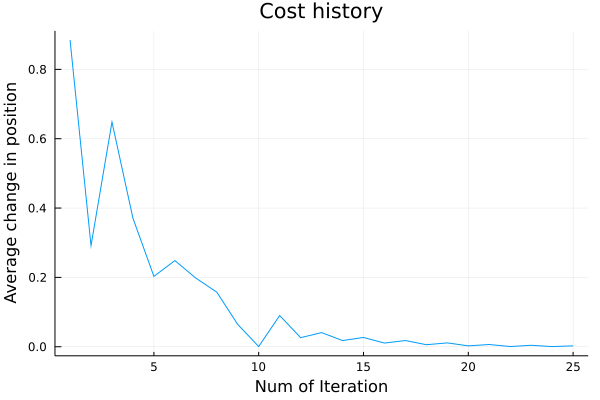
\includegraphics[width=\linewidth]{./plots/CostHistory.png}
\end{center}

\begin{center}
\begin{tabular}{ |c|c|c|c|c|c|c|c|c| } 

\hline
Init(0) & 1 & 2 & ... & 5 & ... & 10 & ... & 25\\
\hline
-8.32 &  0.60 &  0.60 & ... & -0.25 & ... &  -0.21 & ... & -0.0026\\ 
-6.60 &  0.38 &  0.38 & ... & -0.21 & ... &  -0.16 & ... & -0.0021\\  
-4.68 &  0.13 &  0.13 & ... &  0.13 & ... &  -0.08 & ... & -0.0012\\  
-2.33 & -0.16 & -0.16 & ... & -0.13 & ... &  -0.07 & ... & -0.0011\\ 
-0.41 & -0.41 &  0.20 & ... &  0.15 & ... &   0.02 & ... & -0.0001\\  
 1.05 & -0.60 & -0.59 & ... & -0.28 & ... &  -0.09 & ... & -0.0018\\ 
 3.26 & -0.88 & -0.88 & ... & -0.50 & ... &  -0.18 & ... & -0.0051\\ 
 5.10 & -1.12 & -1.12 & ... &  0.00 & ... &   0.00 & ... & -0.0001\\  
 7.16 & -1.38 & -1.38 & ... &  0.04 & ... &   0.04 & ... & -0.0005\\ 
 9.47 & -1.68 & -1.68 & ... &  0.08 & ... &   0.08 & ... &  0.0023\\ 
\hline
\end{tabular}
\end{center}

\subsection{Assumptions in vanilla PSO implementation}

There are numerous variations of PSO and each has it's own constrain. I've made the following assumptions in my implementation.
\begin{enumerate}
  \item Particle initialization: 10 particles were generated uniformly in the range $[-9, 9]$, because we know the objective function is minimum at 0. It is important to make sure generated particles cover the area containing the optimal location otherwise it is difficult for PSO to converge. But sometimes particles are generated in a different area to test a new algorithm. Particle velocity was set to zero. Non zero velocity needs to be set carefully as they may be thrown out of the search space in the first few iterations.
  \item Swarm connectivity: I am using global best - assuming all particles are connected with other particles - similar to a complete graph. Other approaches could involved particles only connected to other particles closer to them based on some measure of distance such as Euclidean distance or spatial similarity.
  \item Control parameters: 
  \subitem Acceleration constant: $s_1$ and $s_2$ are positive acceleration constant that scales the contribution of personal and social component. It was  set to 1.2, where the recommended value is 2. \cite{yang2010engineering}
  \subitem Stochastic parameters: $r_1$ and $r_2$ are sampled from Uniform(0,1) in each iteration \cite{engelbrecht2007computational}. These random values introduces the stochastic behaviour to the particles.
  \subitem Inertia component: The vanilla algorithm is more accurately called `Inertia Weight Variation` because the velocity from the past moment is multiplied by a constant factor or inertia. Van den Bergh and Engelbrecht showed that constant factors need to follow the following relationship to guarantee convergence,
  \begin{equation}
    w > \frac{1}{2}(s_1 + s_2) - 1
    \end{equation}
In our case, $w =0.5$ and $s_1 = s_2 = 1.2$ which satisfies this condition.
  \item Stopping condition: I am assuming the particle will converge after a fixed number of iteration as demonstrated in the example which won't always happen always. We can also stop if the change in average difference in the position of particles falls below an error threshold. We can also look at the slope of a function at candidate positions and stop if the slope is approximately zero (assuming the function is differentiable).
\end{enumerate}


\section{PSO Varients}
The original paper published in 1995 by Kennedy and Eberhart had the following velocity and position update formula for each particle, 
\begin{align*}
v(t+1) &= v(t) + c_1r_1(p_{best} - p_i) + c_2r_2(g_{best} - p_i) \\
x(t+1) &= x(t) + v(t+1) 
\end{align*}
Where $r_1, r_2$ follows $Uniform(0,1)$ velocity is clamped between $[-V_{max}, V_{min}]$ to prevent the particles from flying out of the search space. \cite{kennedy1995particle}. 

PSO is influenced by many parameters such as control parameters, dimension of the problem, number of particles, neighbour hood size(global vs local), number of iterations etc. Some of the variants, their performance and implementation in Python, R and Julia are described below.


\subsection{Inertia Weight}
There is no precise method to chose the range of velocity therefore inertia weight($w$) was introduced by \cite{shi1998modified} to replace velocity clamping which modified the velocity update equation to  
\begin{align*} v(t+1) = \boldsymbol{w} v(t) + c_1r_1(p_{best} - p_i) + c_2r_2(g_{best} - p_i)
\end{align*} and it was also found that the algorithm converges if $w > \frac{1}{2}(c_1 + c_2) - 1$ \cite{van2007analysis}. For w > 1 velocities increase over time, accelerating towards maximum velocity. For w < 1 the particles decelerate until their velocities reach zero. Large values of w facilitate exploration and small facilitate local exploration. But inertia weight could not completely eliminate the need for velocity clamping. weight could also be dynamically by sampling from Gaussian distribution at each iteration, linearly/non-linearly decreasing over time. Alfi and Fateh presented fuzzy PSO where particle dynamically adjust inertia weight according to particle best memories using non-linear model \cite{alfi2011intelligent}.

\subsection{Velocity}

\subsubsection{Velocity clamping}
As velocity increases in each iteration, it is important to clamp its value. If $V_{max}$ is too low swarm may be trapped in local minimum. If it's too high then particle may jump over good region. Usually$V_{max}$ are selected to be a fraction of the search space on each dimension. That is,
\begin{align*}
    V_{max} &=  \delta(x_{max} - x_{min})
\end{align*}
The value of $\delta$ is problem dependent, and we can use cross-validation to find the best value \cite{omran2004image}. A problem arises when all velocities are set to $V_min$ or $V_max$. To solve the problem inertia  weight was introduced as the first solution. Another solution is to change $V_max$ over time linearly or exponentially.

\subsubsection{Velocity constriction}
Clerc  proposed the use of constriction factor similar to inertia weight to balance between exploration and exploitation where velocities are constricted by a constant \cite{clerc1999swarm},
\begin{align*}
\chi &= \frac{2k}{|2-\phi - \sqrt{\phi^2 - 4\phi}|} & \text{where } \phi = c_1 r_1 + c_2 r_2 \text{ and } k \in [0,1]
\end{align*}
This updates the velocity update equation to 
\begin{align*}v(t+1) &= \chi[wv(t) + c_1r_1(p_{best} - p_i) + c_2r_2(g_{best} - p_i)]\end{align*}
Here $\phi > 4$  guarantees convergence. It was developed as an alternate to velocity clamping. $\chi$ is evaluated to the range [0,1] which implies the velocity is reduced in each time step. The term $k$ controls the exploration and exploitation ability of the swarm which is set to a constant value. Furthermore Fan proposed a method where the velocity are multiplied by a scaling factor $(1 - \frac{t}{T})^h$ where t is the number of iteration, T is the maximum number of iteration and h is constant found by trial and error.\cite{fan2002modification} 

\subsection{Particle Connectivity}
The performance of PSO strongly depends on how the particles are connected and how information is flowing through the connection. In a fully connected environment, in original PSO, each particle can learn about the best particle position in the swarm. But particles might be connected to only its neighbour based on some criteria, such as Euclidean distance, spatial similarity etc. This variant do not converge as fast but has more exploitative features. Different social structures have been developed for PSO, such as star, ring, wheel, pyramid, Von-Neumann etc. In Von-Neumann social structure particles are connected in a grid, and it has been found to outperform other social networks in large number of problem. In fully connected structures perform best for uni-modal problem and less connected structure perform better of multi-modal problem \cite{kennedy1999small}.

\subsubsection{Example in Python}
PySwarm implements a local best PSO variant that uses ring topology and locality is defined in terms of distance computed using L2(Euclidean) norm. An implementation where the neighbour size is 3, L2 distance is 2 and running on Rosenbrock function optimized at 0.99 and 0.99 which is what we expected.

\subsubsection{Particle Number and Initialization}
Large number of particles allows larger parts of search space but increase computation time, and mall number of particle lead to insufficient exploration and could result in local optima, and large number of particle are computationally expensive, therefore 20-100 was accepted according to Bratton \cite{bratton2007defining}. It has also been showed that PSO has the ability to find optimal solution with small swarm size of 10 to 30 paticles \cite{bergh2001effects}. 

It is recommended to initialize the velocity of the particles to zero to prevent particles spawned at the edge of the search space to moving out of the search space. Different initialization method has been proposed to ensure the search space is uniformly covered, Sobol sequence \cite{parsopoulos2002particle} and non linear simplex method \cite{parsopoulos2002initializing}. Gehlhaar suggest initializing particles in area that do not contain the minimum can be used to test the ability of the algorithm to find the solution.

\subsection{Stopping Condition}
PSO is an iterative algorithm. A number of termination criteria has been proposed,
\begin{enumerate}
    \item Terminate when maximum number of iteration has been reached. Which is what I used in my Vanilla PSO implementation.
    \item Terminate when an acceptable solution has been found. This requires prior knowledge of the optimal solution. Here we assume $x^*$ is the optimum of the objective function, and the search process stop as soon as we find $x$ which satisfies $f(x) \le |f(x^*) - \epsilon|$. In this method the $\epsilon$ needs to be chosen with care.
    \item Terminate when the particles are clustered up together. In this method we check if all particles are within a $\epsilon$ distance away from the global best particle. If all particles are withing $\epsilon$ when we have a single cluster with all particles which stops the algorithm. It is important to set $\epsilon$ properly to prevent premature terminate.
\end{enumerate}
In some terminating condition, we are expecting the particles to clump up. But the particles could clump up in a local minimum, and we need to be aware of particle converging to local instead of global minimum.

Among many others, Quantum-behaved PSO is an improved upon discrete PSO where the particles movement that is inspired by quantum mechanics. QPSO was further modified to address nullify the influence of outliers during particle movement. QPSO was also modified to have particles memory through a local search before moving.

In some PSO variants both the velocity and position updates rules are substitute. One example is bare-bone PSO where a both rules are substituted by a procedure that samples from a parametric probability density function such as a Gaussian distribution. Adaptive variant of this algorithm changes the standard deviation of the Gaussian distribution. The update rule of PSO was modified to a second order stochastic difference equation by Blackwell \cite{blackwell2011study}

\subsection{Acceleration Coefficient}
Acceleration coefficient $c_1$ and $c_2$ together with $r_1$ and $r_2$ control the stochastic influence of the personal and swarm influence on the velocity of a particle. $c_1$ and $c_2$ are also known as trust parameter. When $c_1 = c_2 = 0$ particle ignore personal and swarm best position keep flying a the current speed until flying out of the search space. If $c_1 > 0$ and $c_2 = 0$ all particles are independent hill climber. If $c_1=0$ and $c_2 > 0$ the entire swarm is attracted to a swarm's best particle.

In most algorithm $c_1$ and $c_2$ coexist in good balance, which means $c_1 \approx c_2$. If $c_1 >> c_2$ particles tends to favor their own personal best over swarm's best. Low values of $c_1$ and $c_2$ result in smooth particle movement and for high values particles make abrupt large movements.

Usually $c_1$ and $c_2$ are static. Suganthan reported that linearly decreasing $c_1$ and $c_2$ has no impact on performance \cite{suganthan1999particle}. Ratnaweera proposed to decrease $c_1$ and increase $c_2$ linearly over time to facilitate early exploration and convergence at the end of the process. The update equations are the following,
\begin{align*}
c_1(t) &=  (c_{1,min} - c_{1, max}) \frac{t}{n_t} + c_{1, max} \\
c_2(t) &=  (c_{2,max} - c_{2, min}) \frac{t}{n_t} + c_{2, min} 
\end{align*}
Where $c_{1, max} = c_{2, max} = 2.5$ and $c_{1, min} = c_{2,min} = 0.5$

For an unconstrained simplified PSO system that included inertia, the trajectory of a particle surely converges if the following condition hold \cite{trelea2003particle},
\begin{align*}
1 > w > \frac{1}{2}(c_1 r_1 + c_2 r_2) -1 \ge 0
\end{align*}
The algorithm might still converge if the condition do not hold.

PSO with time varying acceleration coefficients are also proposed. Cai et al. introduced  time-varying accelerator coefficients which were adjusted according to a predefined predicted velocity \cite{cai2009predicted}. Aminian and Teshnehlab introduced a fuzzy PSO method in which the inertia weight as well as acceleration coefficients were adjusted for each particle separately \cite{aminian2013novel}.


Ni and Deng proposed to use random topology and analyzed its performance. \cite{ni2013new}. Lim and Isa proposed PSO with that linearly increasing topology connectivty with time.

Instead of making the process complex some researcher wanted to simplify standard PSO. For example, Guochu divided the swarm into three categories, better, ordinary and worst particles according to some fitness value \cite{chen2010simplified}.

\subsection{Cognition, Social and Selfless Model}
Also, in PSO variants particles are only affected by their personal best. The velocity update equation is the following,
\begin{align*}
v(t+1) &= v(t) + c_1r_1(p_{best} - p_i)
\end{align*}
Cognition only model is slower in terms of number of iteration required to reach good solution, and it fails when velocity clamping and acceleration coefficient are small. Poor performance of this model was confirmed by  \cite{carlisle2000adapting}.

The social only model ignores the personal best follows the swarm best,
\begin{align*}
v(t+1) &= v(t) + c_2r_2(g_{best} - p_i) 
\end{align*}

It was found that social only model is faster and more efficient than full model in both static and dynamic environment. \cite{kennedy1997particle, carlisle2000adapting}

Selfless model is similar to social model, but instead of using global best, local best is used. Kennedy showed that selfless model to be faster than social only model for few problem \cite{kennedy1997particle}.

\subsection{Discrete}
2 years after the original publication Kennedy \cite{kennedy1997discrete} published a discrete binary version of PSO where the space the particles will explore are discrete. In this modification the velocity update equation remains the same, except the position of particles are represented by 0s and 1s, and the velocity is clamped between [0, 1] which is achieved via logistic transformation $S(v_t) = \frac{1}{1 - e^{v_t}}$. The position update expression was updated,
\begin{equation}
x(t+1) = 
\begin{cases} 
1 & Uniform(0,1) < S(v_{t+1}) \\ 
0 & otherwise 
\end{cases}
\end{equation}
A popular particle swarm optimization Python library is PySwarm that implements discrete PSO.\cite{pyswarms.discrete}

\subsection{Constrained, Multi objective Dynamic Problems}
So far we looked into unconstrained, single-objective, static optimization problems. 

\subssubection{Multiobjectives}
By dynamically updating particle neighbourhood and calculating local best particle position, PSO can be used to address problem that involves multiple objective function. We are interested in generating the Pareto front, which is a set of Pareto optimal solution where it is not possible to improve one objective function without worsening at value of at least one other objective function. In this approach only one objective is optimized at a time. The algorithm used to search for local optima in each generation
is defined as follows:
\begin{enumerate}
    \item Calculate the distances of the current particle from other particles in the fitness value space of the first objective function (not the variable space).

    \item Find the nearest m particles as the neighbors of the current particle based on the distances calculated above (m the neighborhood size).

    \item Find the local optima among the neighbors in terms of the fitness value of the second objective function.
\end{enumerate}

\subsubsubsection{Example in R}
MOPSO-CD is a variant of multi-objective PSO that uses crowding distance(CD) computation to ensure an even spread of non-dominated solutions. Here in an example in R optimizing Viennet function\cite{irfan_2021}.

\subsubsection{Constrains}
Particles might move to region that is not feasible, and PSO variants were developed to handle situations like that. Some very simple approaches are, 
\begin{enumerate}
    \item If the number of infeasible particles are small, not allowing those  particle to be selected as personal or global best could result in them being pulled back in the feasible space.
    \item Reject infeasible particles and replace them with newly generated ones.
    \item Add penalty for infeasible particles \cite{parsopoulos2002particle}. 
    \item Apply repair operation on the feasible particles to move them back to feasible space. Hu and Eberhart developed an approach where particles are not allowed to be attracted by infeasible particles. \cite{hu2002solving}
\end{enumerate}

An example in written in R that is running PSO with inertia weight on 1 objective function and 4 constrains. Each time the particle position do no satisfy constrain, a penalty value (1000) is added to it \cite{irfan_2021} Section 3.

Yang \cite{yang2011particle} proposed PSO with modified velocity startegy in which each particle was attracted by global best particle and a random particle chosen from a set of good particle, and this setup perfomed beter than standard PSO.Wang et al. [196] compared and analyzed the optimization performance of PSO under different parameters, in order to guarantee the convergence of PSO applied to the inverting of ellipsometry. The result showed that the range of inertia weight omega from 0.5 to 0.8, the sum of learning parameters c1 and c2 preferably no more than 3, and a smaller c1 and a bigger c2 ensured the better optimization performance of PSO.


\section{Show usage of MLJ Library}
For example: What for example might be included in the state object that gets passed around by the various methods (the API is basically “functional” in style)?

Pending: I am currently going through the tutorials at \url{https://alan-turing-institute.github.io/DataScienceTutorials.jl/}
 to familiarize myself with MLJ and MLJTuning.

\pagebreak

\printbibliography
\end{document}